\documentclass{deliverablereport}

\usepackage[style=alphabetic,backend=bibtex]{biblatex}
\addbibresource{../../lib/kbibs/kwarc.bib}
\addbibresource{rest.bib}
% temporary fix due to http://tex.stackexchange.com/questions/311426/bibliography-error-use-of-blxbblverbaddi-doesnt-match-its-definition-ve
\makeatletter\def\blx@maxline{77}\makeatother

\usepackage{tikz}
\usetikzlibrary{positioning}
\usetikzlibrary{shapes.geometric}
\usetikzlibrary{shadows}
\usetikzlibrary{patterns}
\usetikzlibrary{arrows}
\usetikzlibrary{backgrounds}
\usetikzlibrary{mmt}
\usetikzlibrary{tikzmark}
\usetikzlibrary{decorations,decorations.markings,decorations.text,decorations.pathmorphing}
\usepackage{standalone}
\usepackage[show]{ed}
\usepackage{listings}
\lstset{columns=fullflexible,basicstyle=\sf,language=Python}
% Variant: we could just provide the deliverable label as in the
% proposal, and fetch all the information from final.pdata

\deliverable{UI}{adstex}
\deliverydate{27/06/2016}
\duedate{05/31/2016 (Month 6)}
\def\pn{OpenDreamKit}
\author{Michael Kohlhase}

\begin{document}
\maketitle
%  Work Package WP6 develops a novel, foundational, knowledge-based framework for
  interfacing existing open source mathematical software systems and knowledge bases into
  a mathematical VRE, where systems can delegate functionalities among each other
  seamlessly without losing semantics.

  The overall Math-in-the-Middle (MitM) Framework developed in WP6 over the last three
  years is described in D6.5; this Report complements it by describing the curated
  contents Math-in-the-Middle (MitM) Ontology which serves as a reference and pivotal
  point for translations between the various input languages of mathematical software
  systems and knowledge bases.

  In a nutshell, the MitM Ontology describes the mathematical objects, concepts, and their
  relations in a general, system-agnostic way in an OMDoc/MMT theory graph while the
  mathematical systems export API theories that describe the system interface language in
  terms of types, classes, constructors, and functions -- again in OMDoc/MMT. These two
  levels of descriptions are linked by OMDoc/MMT alignments that allow the translation of
  expressions between systems.

%%% Local Variables:
%%% mode: visual-line
%%% fill-column: 5000
%%% mode: latex 
%%% TeX-master: "report"
%%% End:

\strut\githubissuedescription
\newpage\tableofcontents\newpage

\section{Introduction}\label{sec:intro}

\begin{newpart}{MK: adapted from Tom's Thesis}
There is a large and vibrant ecosystem of open-source mathematical software systems.
These systems can range from calculators, which are only capable of performing simple
computations, via mathematical databases (curating collections of a mathematical objects)
to powerful modeling tools and computer algebra systems (CAS). 

Most of these systems are very specific -- they focus on one or very few aspects of
mathematics.  For example, the ``Online Encyclopedia of Integer Sequences''
(OEIS~\cite{Sloane:oeis12,oeis}) focuses on sequences over $\mathbb{Z}$ an their
properties and the ``L-Functions and Modular Forms Database''
(LMFDB)~\cite{Cremona:LMFDB16,lmfdb:on} objects in number theory pertaining to Langland's
program.  GAP~\cite{GAP:on} excels at discrete algebra, whereas
SageMath~\cite{SageMath:on} focuses on Algebra and Geometry in general, and
Singular~\cite{singular:on} on polynomial computations, with special emphasis on
commutative and non-commutative algebra, algebraic geometry, and singularity theory.

For a mathematician however (a user; let us call her Jane) the systems themselves are not relevant, instead she only cares about being able to solve problems. 
Typically, it is not possible to solve a mathematical problem using only a single program. 
Thus Jane needs to work with multiple systems and combine the results to reach a solution. 
Currently there is very little help with this practice, so Jane has to isolate sub-problems the respective systems are amenable to, formulate them into the respective input language, collect results, and reformulate them for the next system a tedious and error-prone process at best, a significant impediment to scientific progress in its overall effect. 
Solutions for some situations certainly exist, which can help get Jane unstuck, but these are ad-hoc and for specific, often-used system combinations only. 
Each of these requires a lot of maintenance and does not scale to a larger set of specialist systems. 

The OpenDreamKit project, which aims at a mathematical VRE toolkit, proposes the Math-in-the-Middle (MitM~\cite{DehKohKon:iop16}) Paradigm, an interoperability framework based on a flexiformal
representation of mathematical knowledge and aligns this with system-generated interface
theories. 

In this paper we instantiate the MitM paradigm with a concrete domain development and
evaluate it on a distributed computing GAP, SageMath and Singular.\ednote{ we generally we
  want to show that the promises in the CICM paper become reality.}

We will use the following example as a running example: Jane wants to act on singular
polynomials with GAP permutation groups\ednote{MK@(MP|VA): }

 \ednote{MK: continue with the structure} 
\end{newpart}

%%% Local Variables:
%%% mode: latex
%%% TeX-master: "paper"
%%% End:
\newpage
%\subsubsection{Jupyter}
\label{sec:jupyter}

\begin{wrapfigure}{r}{0.50\textwidth}
%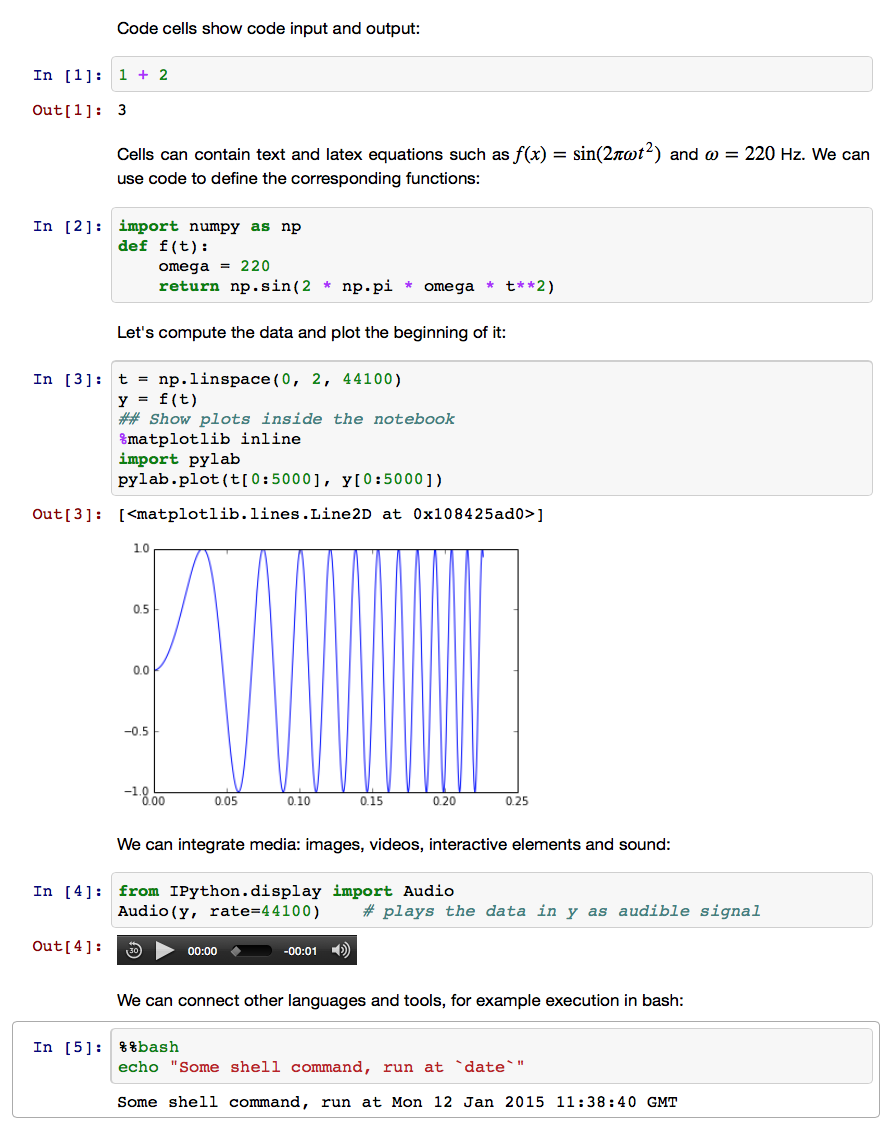
\includegraphics[scale=0.23]{Pictures/jupyterdemo1.png}
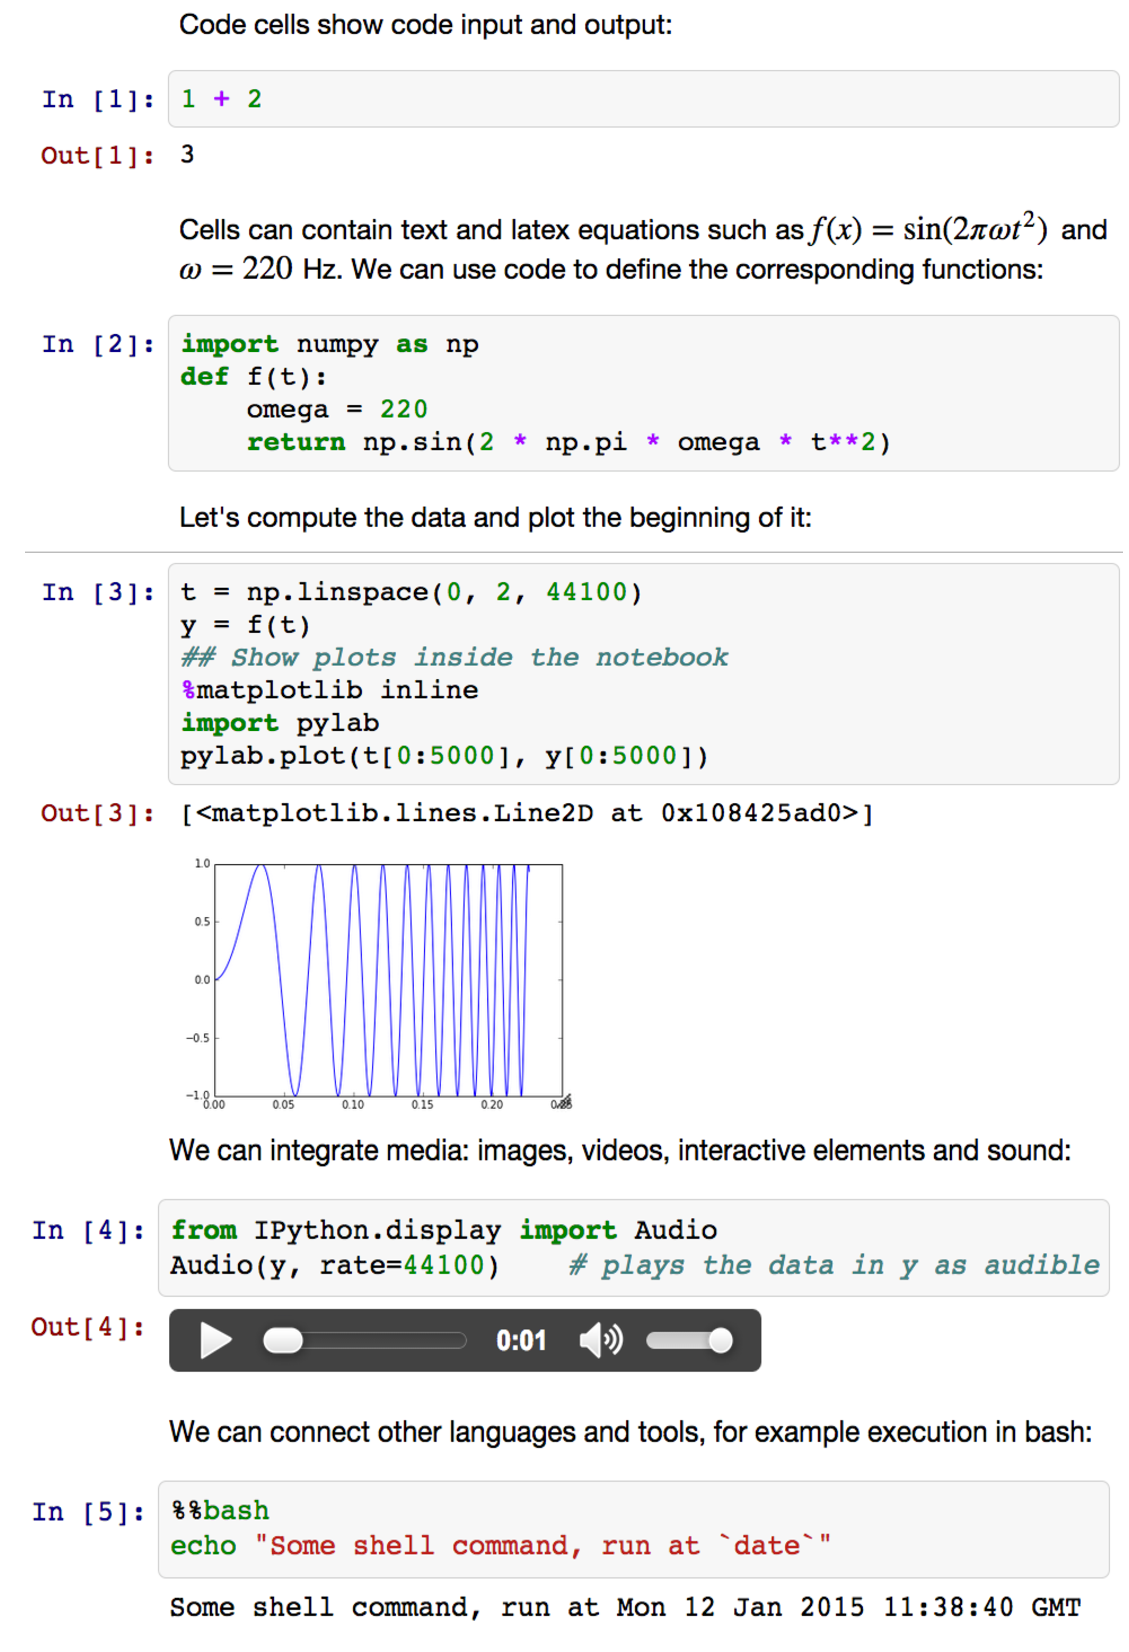
\includegraphics[width=.5\textwidth]{Pictures/jupyterdemo-largefont.pdf}
\caption{\label{fig:jupyterdemo} Self-contained \Jupyter Notebook demonstrating the concepts of cells that contain different types of material and can be executed (or updated) in arbitrary or sequential order.}
\end{wrapfigure}

Project \Jupyter \cite{Jupyter} is a set of open-source software projects for
interactive and exploratory computing emerging from \IPython \cite{IPython}. These
software projects help make scientific computing and data science
reproducible and multi-language (Python, Julia, R, Haskell, Bash, R,
\ldots). The main component offered by \Jupyter is the \Jupyter
notebook, a web-based interactive computing platform that allows users
to create data- and code-driven narratives that combine live
(re-executable) code, equations, narrative text, interactive
dashboards and other rich media.

Figure~\ref{fig:jupyterdemo} shows a Python-based sample
session. Within the Python session, all libraries available in Python
can be imported and combined flexibly, a number of interfaces between
different languages exist. Many more examples are available, for
example \cite{IPython-demo-hyperbolic-conservation-laws} and
within \cite{IPython-sload-foundation-report-2013}.

The \Jupyter notebook is being used widely in academia
(e.g. University of California, Berkeley, Stanford,
MIT, Harvard, Cambridge, Oxford, Imperial College, Southampton,
Hamburg, Paderborn, Vienna, Paris, Katowice, and Oslo) and government
(NASA JPL, LBL, KBase, White House Hackathon) as well as
industry (e.g. Google, IBM, Facebook, Oracle, Otto Group, Microsoft,
Bloomberg, JP Morgan, WhatsApp, O’Reilly, Quantopian, Logilab,
GraphLab, Enthought, Continuum, Authorea, BuzzFeed)  and
journalism (e.g. 538 and New York Times). \\
%
Because the architecture and building blocks of \Jupyter are open,
they are used to build numerous other commercial and non-profit
products and services. The \Jupyter Notebook has between 500,000 and
1.5 million individual users worldwide.

These notebook documents provide a \emph{complete} and
\emph{executable} record of a computation that can be shared with
others in a way that has not been possible before. This has led, among
other things, to a huge boost in reproducible, interactive
teaching/education documents in recent years. A paradigm that Fernando Perez, creator of the project, has referred to as ``literate computing''.\footnote{\url{http://blog.fperez.org/2013/04/literate-computing-and-computational.html}}

We will build on this technology by extending \Jupyter with new
functionality, unifying other computational tools to be usable as
components in this framework, and merging the \Sage and \Jupyter
development.  \TOWRITE{NT}{Is the 'merge' too strong a claim? Please
  correct / remove.}



\newpage
\section{Active Documents}\label{sec:active}
\def\mathhub{MathHub.info\xspace}
\def\mmt{MMT\xspace}
\def\ommt{OMDoc/MMT\xspace}
\def\imgdir#1{#1}
\subsection{Introduction}

We define the Active Documents as semantically annotated documents associated with a
content commons that holds the corresponding background ontologies. An \textit{Active
  Document Player} embeds user-visible, interactive services like program execution,
computation, visualization, navigation, information aggregation and information retrieval
to make documents executable. We call this framework the Active Documents Paradigm (ADP;
see Figure~\ref{fig:activedocs}), since documents can also actively adapt to user
preferences and environment rather than only executing services upon user request. The ADP
is implemented in the Active Documents Portal MathWeb.info~\cite{MathHub:on} building on
standard components as an instance of the Planetary system \cite{Kohlhase:ppte12}; see
Section~\ref{sec:mathhub:arch} below.

\begin{figure}[ht]\centering
  \documentclass{standalone}
% \usepackage[mh]{mikoslides}
% % this file defines root path local repository
\defpath{MathHub}{/Users/kohlhase/localmh/MathHub}
\mhcurrentrepos{MiKoMH/talks}
\libinput{WApersons}
% we also set the base URI for the LaTeXML transformation
\baseURI[\MathHub{}]{https://mathhub.info/MiKoMH/talks}

% \libinput{preamble}
\usepackage{tikz}
\usetikzlibrary{positioning}
\usetikzlibrary{shapes.geometric}
\usetikzlibrary{shadows}
\usetikzlibrary{patterns}
\usetikzlibrary{arrows}
\usetikzlibrary{backgrounds}
\usetikzlibrary{mmt}
\usetikzlibrary{tikzmark}
\usetikzlibrary{decorations,decorations.markings,decorations.text,decorations.pathmorphing}
\begin{document}
\begin{tikzpicture}
[inner sep=1.5mm, node distance=2cm,outer sep = 0pt,
place/.style={circle,draw=blue!50,fill=blue!20,thick,outer sep = 0pt},
transition/.style={regular polygon,regular polygon sides=4,draw=blue!50,fill=blue!20,thick},
dblock/.style={rectangle, draw, fill=blue!20, 
    text width=4em, text centered, minimum height=3.5em},
wblock/.style={rectangle, draw, fill=blue!20, rounded corners,
    text width=5em, text centered, minimum height=3.5em,outer sep=4pt},
scale=1.4]

%% the diagram, which is also defines the origin
\node (center) at (0,0) [place] {};
\node (middleleft) at (-1.5,0) [transition] {};
\node (middleright) at (1.5,0) [transition] {};

\node (righttop) at ( 1,1) [place] {};
\node (lefttop) at (-1,1) [place] {};b

\node (leftbottom) at (-1,-1) [place] {};
\node (rightbottom) at (1,-1) [place] {};

%% labels
\coordinate (A) at (-2.5,5);
\coordinate (B) at (-2.5,-1.5);
\coordinate [label=left:{Document Commons}] (C) at (-3,4.8);
\coordinate [label=right:{Content Commons}] (D) at (-2,4.8);
\node[text width=4em] at (2.5,1.2) {Content Objects};

%% lines

\draw[-] (center) -- (lefttop);
\draw[-] (center) -- (rightbottom);
\draw[-] (center) -- (leftbottom);
\draw[-] (center) -- (righttop);
\draw[-] (lefttop) -- (righttop);
\draw[-] (leftbottom) -- (rightbottom);
\draw[-] (leftbottom) -- (middleleft);
\draw[-] (middleleft) -- (lefttop);
\draw[-] (middleright) -- (righttop);
\draw[-] (middleright) -- (rightbottom);
\draw[->,dashed] (lefttop.north) to [bend left=45] (righttop.north);
\draw[->,dashed] (leftbottom) -- (lefttop);

\draw[-,dashed] (A) -- (B);

%% active documents and player
\node (activedocs) at (-5,0) [dblock] {Semantic Documents};
\node at (-4.6,0.4) [dblock] {Semantic Documents};
\node at (-4.8,0.2) [dblock] {Semantic Documents};
\node at (-5,0) [dblock] {Semantic Documents};

\node (player) at (-2.5,3.2) [wblock] {Active Document Player};
\node[draw,left=3cm of player] (user) { User };
\draw[<->,draw,dashed] (player) -- node[above]{view} node[below]{interact} (user);

\draw[<->,draw,thick] (-1.5,0) -- (-3.5,0);
\draw[<->,draw,thick] (-4.5,1.1) -- (-3.5,2.5);
\draw[<->,draw,thick] (-.3,1.1) -- (-1.5,2.5);
\end{tikzpicture}
\end{document}

%%% Local Variables:
%%% mode: latex
%%% TeX-master: t
%%% End:

  \caption{Active Documents}\label{fig:activedocs} 
\end{figure} 

We present the ADP with a focus on three distinct annotation levels, \textit{presentation
structure}, \textit{semantic} and \textit{formal}.

\subsection{Presentation Structure}

The importance of the presentation structure level is that an active document player can
turn legacy documents into active documents by transforming them into
XHTML+MathML+SVG-encoded documents with semantic annotations in RDFa.

We have transformed over half a million articles from the Cornell ePrint arXiv to
XHTML+MathML with LaTeXML, preserving properties like document and formula structures and
embedded them into an instance the Planetary System, an active documents player.

The document structure can then be exploited for a FoldingBar service (see on the left in
Figure~\ref{fig:interacting-article}) and for localizing discussions about document
content to document structures and subformulae – e.g. for questions/answers, or reviewers'
comments. In the situation in Figure 6 we have clicked on the formula, which pops up the
IconMenu with three options: reporting errors in the content (bug icon), asking/answering
a question (question mark icon), and accessing the discussion threads of this element
(balloons icon). Here, a click on the question mark icon allowed us to pose a question and
hope for an answer by other users in the forum. Figure 6 also shows the Planetary InfoBar
with information markers on the right, which indicate the availability and state of the
discussion threads pertaining to information objects in the line they are horizontally
aligned with. Clicking them will highlight all items that have discussions. Localized
discussions have proven a very valuable tool for community-based validation of papers,
especially if they are coupled with a discussion subscription/trackback system for readers
and personal notification system for authors.

\begin{figure}[ht]\centering
    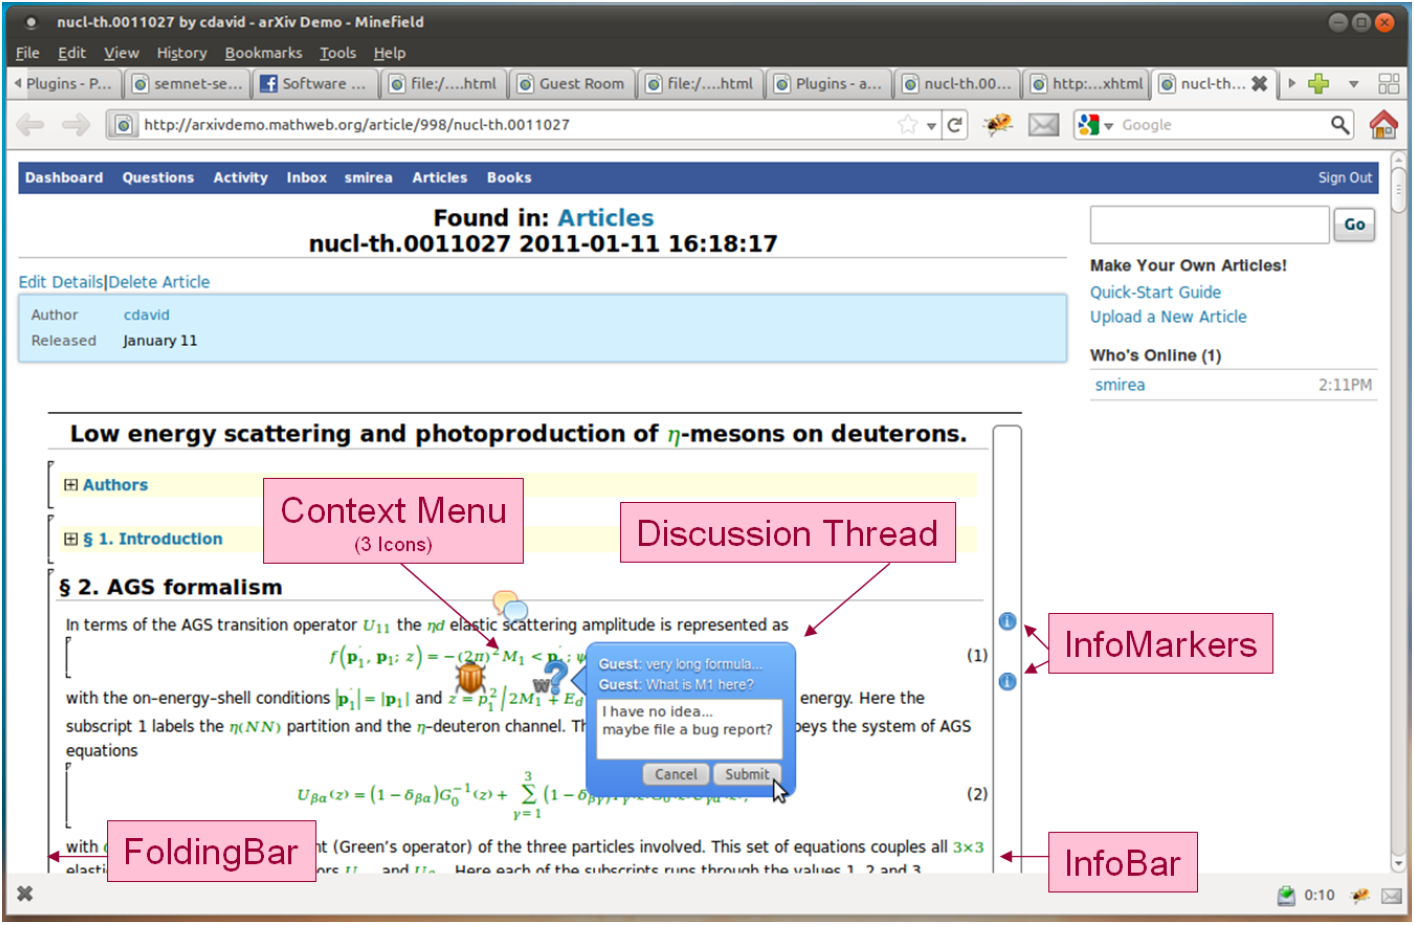
\includegraphics[width=\textwidth]{PresentationStructure}
    \caption{Interacting with an article}\label{fig:interacting-article}
\end{figure} 

\subsection{Semantic Level}

We can considerably improve the user experience by extending the depth of semantic
annotations. For this we employ OMDoc (Open Mathematical Documents), an XML-based
content-oriented, semi-formal representation format for scientific and technical documents.

It builds on the OpenMath/MathML3 semantic representation format for mathematical formulae. OMDoc extends OpenMath with an infrastructure for context and domain models from
Formal Methods, as well as a generic document infrastructure. At the semantic level
Planetary is based on STEX documents, which can be transformed to OMDoc and via a
user-adaptive and context-based presentation process further to XHTML+MathML+SVG+RDFa. The
generated OMDoc documents are committed to an instance of the versioned XML database
TNTBase that indexes them by semantic functional criteria, and can then perform
server-side semantic services via user-defined XQuery queries.

\begin{figure}[ht]\centering
  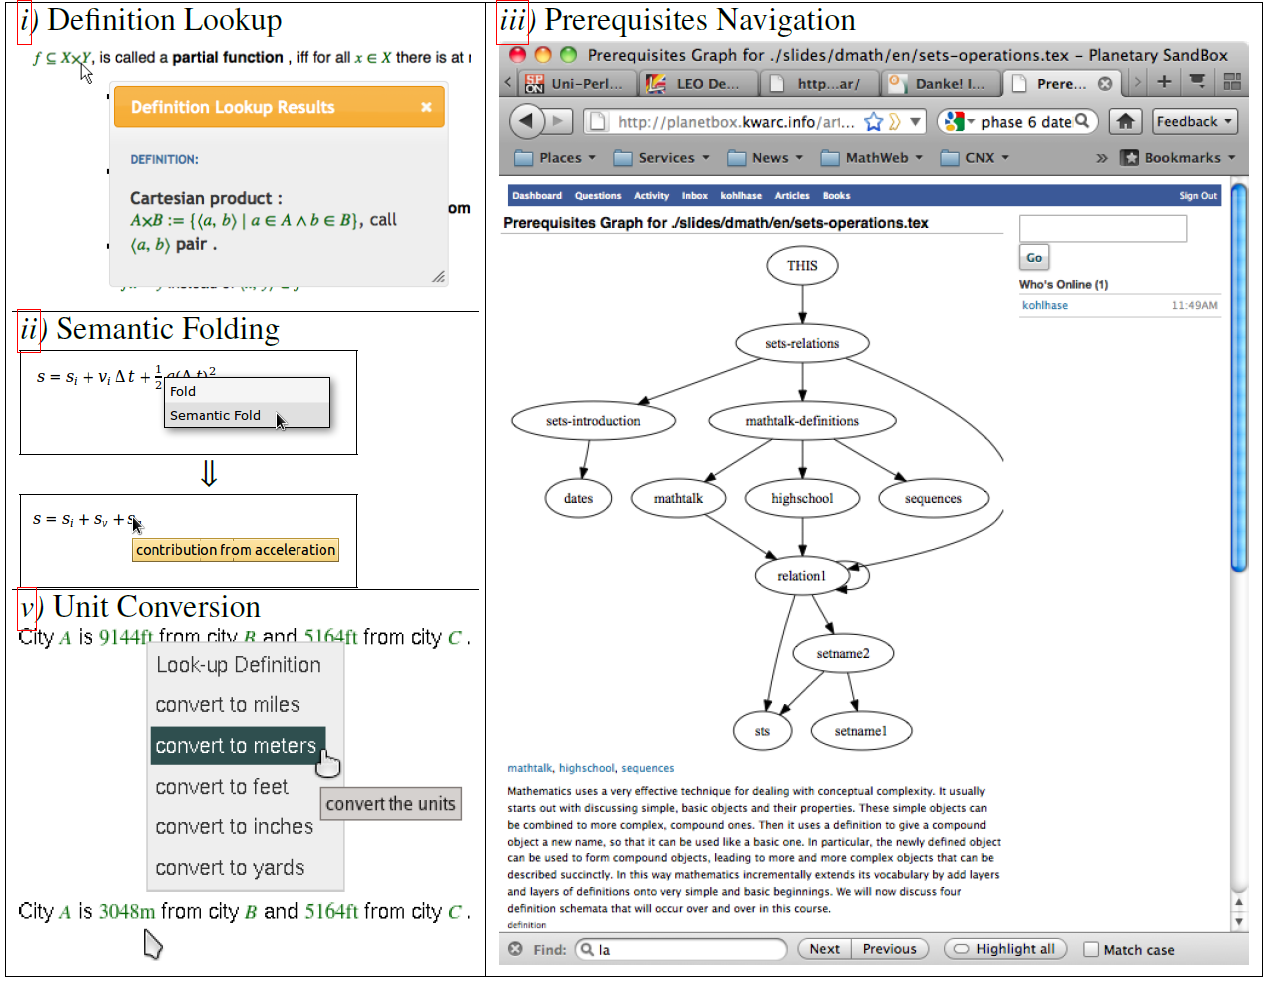
\includegraphics[width=\textwidth]{UserServices}
  \caption{User Services at the Semantic Level}\label{fig:adt:semantic} 
\end{figure} 

TNTBase thus becomes a source of the user-adaptive, custom-generated documents forming
Planetary's content commons. Many semantic services can directly be derived from this setup. At the semantic level, the IconMenu we know from Figure 6 can be extended,
depending on the services available for the semantic item in focus. The book icon triggers
definition lookup (see item i) below) and the graph and portrait icons prerequisites
navigation (see iii)). Figure 7 shows results of these and other services.

\begin{enumerate}
\item \textit{Definition Lookup}: All technical terms and symbols in formulae presented in
  Planetary are linked to their semantic counterparts in the content commons, which in
  turn are linked to their definitions.
\item \textit{Semantic Folding}: If any explanations of the meanings of subformulae have
  been added as annotations, folding can use these instead of ": : :". In Figure 6/ii) the
  motion law above is semantically folded to \[s_0 + s_v + s_a \]
  and the abbreviations \[s_*\] are explained via flyover help.
\item \textit{Prerequisites Navigation}: As the content commons has an inherent notion of
  semantic dependency, we can use that to show prerequisites leading to a
  concept. Currently Planetary supports two ways of dealing with prerequisites: i) a
  concept graph view, where the required concepts can be navigated on demand by clicking
  on concept nodes, and ii) guided tours, where the necessary content is generated in a
  coherent narrative.
\item \textit{Executable Formulae}: As the formulae in the documents are generated from
  OpenMath objects, we can export them to a computer algebra system like Mathematica (or
  in our case the open-source system GAP, which has been made available as an
  OpenMath-based Web service) for evaluation, graphing, or experimentation.
\item \textit{Unit Conversion}: In scientific papers, formulae often contain expressions
  for measurable quantities; these can be automatically converted to other unit systems.
\end{enumerate}

Note that the underlying OMDoc format and the services based on it address a peculiarity
of documents in the STEM disciplines. Here, documents are dynamic in the sense that they
declare new concepts, definitions, model assumptions, terminology, notations, etc., as
they go along, or else they explicitly (or implicitly) import such items from other
documents. As a consequence, all knowledge items in STEM documents have a non-trivial
context of declarations. This must be managed explicitly in our representations of these
documents, in the content commons, and within user interaction in order for semantic
services to be effective. This effect is especially pronounced in mathematical sciences
(including Computer Science, Physics etc.), and somewhat less so in Chemistry and the Life
Sciences, where a global context in the form of external terminology and notation
databases often suffices.

\subsection{Formal Level}

Finally, we can use Planetary as a frontend system for completely formal content. OMDoc is
also a foundation-agnostic integration format for mathematical knowledge that can express
web ontologies, program specifications and verifications, and even representations of
logics in logical frameworks like LF. In formal systems, documents are dominated by
complex formulae, and users need support in navigating, abstracting, and evaluating them
in order to cope with this complexity. Figure 8 shows how fully formalized formulae can be
adapted to user preferences, about, e.g., the level of brackets and the availability of
inferred arguments or definitions. Further semantic services at the fully formalized level
include access to automated theorem provers via the HETS system and argument
reconstruction via the Twelf system.

It is important to note that programs (and program fragments) are also knowledge items at
the fully formal level, as all their semantics can be recovered by parsing. Program
fragments are not yet supported by Planetary.

\begin{figure}[ht]\centering
  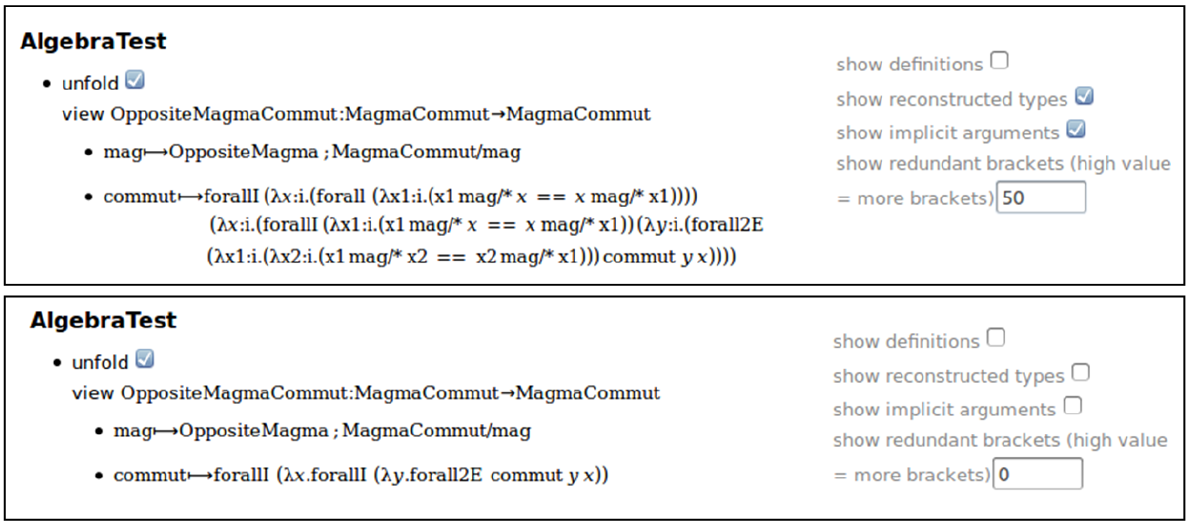
\includegraphics[width=\textwidth]{FormalRepresentationAdapted}
  \caption{Formal Representations Adapted to Distinct User Settings (Customized via the
    DocDash Widget on the Right)}
\end{figure} 

\subsection{Architecture}\label{sec:mathhub:arch}
\mathhub has four main components (see Figure~\ref{fig:arch}):
\begin{compactenum}[\em i\rm)]
\item a versioned \emph{backend} holds the libraries,
\item the \mmt API as the kernel tool understands the libraries provides semantic services
  for them,
\item a web-based \emph{frontend} makes the libraries and services available to users,
\item a Javascript \emph{plugin architecture} enriches document presentations with
  localized semantic services.
\end{compactenum}
We use best-of-breed open source systems for the components going beyond \mmt.  In the
backend, we use GIT for versioning, distribution, and user/rights management adapting the
GitLab repository manager~\cite{GitLab:on}, an open-source alternative to GitHub. For the
frontend, we use the Drupal container management system.\footnote{Drupal and similar
  systems self-describe as ``content management systems'', but they actually only manage
  the documents and their metadata -- essentially document containers -- without changing
  their internal structure.} For the Javascript library we use our JOBAD framework
\cite{GLR:WebSvcActMathDoc09,Kohlhase:ppte12}, which embeds semantic services into HTML
documents and thus makes them interactive and user-adaptive.  Even though JOBAD is just a
relatively thin layer of glue code that picks up on semantic annotations in the generated
HTML5, its effect for the users is rather profound: It gives them access to added-value
services ``at the point of pain/interest'', i.e., in the user interface.
Figure~\ref{fig:adt:semantic} already shows JOBAD in action: it links fragments of the
formula presentations with computations in the \mmt system and makes both available to the
user embedded in the document.

\begin{figure}[ht]\centering\def\imgdir{img}
  \documentclass{standalone}
\usepackage{tikz}
\usetikzlibrary{positioning,shapes,shapes.geometric,docicon,arrows}
\newcommand{\omdoc}{OMDoc}
\begin{document}
\providecommand\myxscale{1}
\providecommand\myyscale{1}
\providecommand\imgdir[1]{#1}
\providecommand\myfontsize{\normalsize}
\begin{tikzpicture}[xscale=\myxscale,yscale=\myyscale]\myfontsize\sf
  \pgfdeclareimage[width=1cm]{user}{user}
  \pgfdeclareimage[width=1cm]{author}{author}
  \tikzstyle{system} = [rectangle, draw, fill=blue!20, text width=1.1cm, text centered,
                                    rounded corners, minimum height=.8cm,shade, 
                                    top color=white, bottom color=blue!20]
   \tikzstyle{database} = [cylinder,cylinder uses custom fill,
      cylinder body fill=yellow!50,cylinder end fill=yellow!50,
      shape border rotate=90,
      aspect=0.25,draw]
\node (user) {\pgfuseimage{user}}; 
\node[system,right=1.2cm of user] (browser) {Browser}; 
\node[system,right=1.1cm of browser] (drupal) {Drupal};
\node[system,above right=0cm and 1.4cm of drupal] (mmt) 
            {\hspace*{-.5em}\begin{tabular}{c}MMT\\System\end{tabular}};
\node[system,below right=0cm and 1.4cm of drupal] (gl) {GitLab};
\node[database,below right=.3cm and .7cm of gl] (lib) {library};
\node[right=1.6cm of gl] (author) {\pgfuseimage{author}}; 
\node[below right=-.5cm and .6cm of mmt] (conv) 
            {\begin{tabular}{l}\footnotesize convert source to\\ OMDoc/MMT\end{tabular}};
\node[system,below=.8cm of drupal] (mws) {MWS};
\draw[->,thick] (mws) -- node[above] {harvest} (gl);
\draw[->,thick] (drupal) -- node[left] {query} (mws);
\draw[<-,thick] (mmt) -- node[left]{load} (gl);
\draw[<->,dotted] (user) -- node[above]{casual} node[below]{user} (browser);
\draw[->,thick] (browser) -- node[above]{REST} (drupal);
\draw[->,thick] (browser) to[loop above] node [above] (jobad) {JOBAD} (browser); 
\draw[->,thick] (gl) to[loop left,out=20,in=45,looseness=14] (gl); 
\draw[<->,dashed] (jobad) -- (mmt);
\draw[<->,dashed] (conv) -- (mmt);
\draw[<-,thick] (drupal) -- node[above=.1cm]{semantics}(mmt); 
\draw[->,thick] (drupal) -- node[above]{edit}(gl); 
\draw[<->,dotted] (author) -- node[above]{power} node[below]{user} (gl);
\draw[->,dotted] (lib) -- node[left]{import} (gl);
\end{tikzpicture}
\end{document}
%%% Local Variables:
%%% mode: latex
%%% TeX-master: t
%%% End:

  \caption{The modular \mathhub Architecture}\label{fig:arch}
\end{figure}
Figure~\ref{fig:arch} shows the detailed architecture.  Here GitLab provides distributed
versioned storage of the libraries and organizes them into repositories owned by users and
groups.  And Drupal supplies uniform theming, discussion forums, and a plugin
infrastructure for adding interface functionality.  Both systems provide user management,
but we automatically synchronize the users and permissions between them, so that GitLab
becomes invisible to the casual user.

This componentized architecture has the advantage that we can combine two methods for
accessing the contents of \mathhub:
\begin{inparaenum}[\em i\rm)]
\item an online, web-based workflow for the casual user, and
\item an offline authoring workflow based on git working copies for power users and bulk
  edits.
\end{inparaenum}
Users can fork or pull the relevant repositories from GitLab, edit them, and submit them back to \mathhub
either via a pull request to the repository masters or a direct commit/push.
As the content is often highly interlinked and distributed across multiple interdependent repositories, we
have developed tool support for managing multiple working copies across repository borders.

In the web-based system, semantic services (notation-based, presentation, definition
lookup, relational navigation, dependency management, etc.) are provided by \mmt and are
made available to the user, primarily by dedicated JOBAD~\cite{GLR:WebSvcActMathDoc09}
modules.
The interactive functionalities in \mathhub are based on the \ommt representation of
the libraries, but authors and users have to interact with them in the respective source
language of the library.  Both the source and \ommt representations are versioned in
GitLab and the respective source representations must be converted into \ommt by
language-specific custom exporters. Correspondingly library import is managed by \mathhub
at the level of the GitLab repository.

Then we can dedicate a specific GIT working copy together with an \mmt instance to a user
or a group that shares permissions.  Thus, the \mmt instance sees (and takes into account
for its services) only the documents accessible to the group.  If an authenticated user
edits \mathhub content, the changes are committed under his name into the specific working
copy.  This makes it easy to cope with multiple synchronous users, for which \mathhub uses
separate working GIT clones and \mmt instances.


\subsection{Conclusion}

The Active Documents stand for semantically annotated documents connected to a content
commons accessed through an adaptive document player , such as Planetary. The Planetary
system is presented as an answer to the challenge of creating "executable papers". We have
shown the initial feasibility of the concept in a variety of publicly available case
studies.

Along the Planetary system, the Active Documents addresses all the following challenges:

\begin{itemize}
\item \textbf{Executability} is achieved by an extensible and configurable collection of
  semantic services that can be embedded into documents. In particular, code can be made
  executable via external computation machines, and computational experiments can be
  repeated and varied (via the same mechanism). Where the functionality of a service
  depends on ontologies, the user community can customize the service by customizing the
  ontology inside Planetary.
\item \textbf{Short and long-term compatibility} is guaranteed by usage of open standards
  in representation formats and protocols (XML, RDF/RDFa, OpenMath, MathML, XQuery,
  SPARQL, XHTML, SVG) supporting a web service framework, and hence
  operating-system-independent. Of course, Planetary can export monographs, collections
  and even entire libraries both as PDF (inactive documents) or in the EPUB eBook format.
\item \textbf{Validation} and in particular human refereeing and scientific validation can
  be facilitated via an in-text discussion feature. Moreover, documents can be
  automatically validated via semantic services, e.g. automated SI-dimensionality
  checking.
\item \textbf{Copyright/licensing} is represented by fine-grained RDFa-based metadata
  annotations in STEX and OMDoc, which are maintained over the presentation process. So
  they can be used for filtering or attribution either on the backend storage level
  (TNTBase, RDF triple store) or in the frontend Planetary system. Together with the user
  management and permission system, Planetary can be extended to enforce compliance. In
  fact, as documents are assembled for the user at view-time they can be adapted to the
  license status of the user (e.g. it is possible to make a document license conforming by
  leaving out examples that are not licensed to her specific institution).
\item \textbf{Systems} As the Planetary system is entirely based on web standards and
  communicates via RESTful interfaces, it is simple to wrap external systems into web
  services, if we can equip them with OMDoc, OpenMath, or RDF interfaces.
\item \textbf{Size} Even though individual human-written documents are modest in size,
  journals and encyclopedias can get big – consider e.g. the Wikipedia or the arXiv. The
  Planetary system has been tested on the latter; the underlying data stores scale
  sufficiently for large document collections. Furthermore, the modular and semantic
  document formats accommodate the integration of external data stores via 'special'
  links, which the Planetary player can interpret on view, hence keeping the storage
  minimal and the experience optimal. To the best of our knowledge, the semantically
  transparent integration of data into a document player application is a new feature of
  the Planetary system.
\item \textbf{Provenance} comes in various aspects. Data provenance can be specified by
  the techniques for semantic integration of data fields. For instance we can specify
  units (as OpenMath objects) and computations to obtain the displayed data from raw data,
  etc. As all of these are content representations in the documents or the content
  commons, they can be handled with semantic services. The system state provenance
  (i.e. what actions of the user led to the current state of interaction in the Planetary
  system), can be handled by recording system data ("who did what when") in the metadata
  store of Planetary. This can be opened to querying the system ontologies we have
  developed for semantically transparent system self-documentation. An encouraging aspect
  of this work is that document authors only need expertise in their own domain. In
  particular, no system-level programming is necessary for authors: the semantic
  representation formats involved act as a high level conceptual interface between content
  authors and system/service/interface developers. We are convinced that without such a
  separation of concerns, "the next generation of publishing" will not scale enough to
  become practical.
\end{itemize}

%%% Local Variables:
%%% mode: latex
%%% TeX-master: "report"
%%% End:
\newpage
\section{A Joint Perspective and Generalization of Jupyter and Active
  Documents}\label{sec:comparison}

We will now highlight the features of the ADP and Jupyter notebooks with a view towards a
possible unification of the systems.

\begin{figure}[ht]
  \documentclass[border = 120pt]{standalone}

\usepackage[landscape]{geometry}
\usepackage{tikz}
\usetikzlibrary{mindmap}
\usepackage{metalogo}
%\usepackage{dtklogos}
\usetikzlibrary{shapes, snakes}
\begin{document}
\begin{tikzpicture}[xscale=.9]

%Mother Ship
\draw[fill=blue!10] (-9,-3.5) rectangle (-15, 4.5);

%Active Document
\node[align=center, text width=5cm] at (-12,4) {\textbf{This is an example title}};
\node[align=left, text width=5cm] at (-12,2.5) {This is a sentence used to represent the interactivity between the text and the active document.};
\draw[style=thick, fill=cyan] (-14, 1.5) rectangle (-11.25, 1);
\node[align=left, text width=5cm] at (-11,1.25) {Interactivity.};

\node[align=left, text width=5cm] at (-12, 0) {Among the text of an active document there are fields which can interact with the user such as:};
\draw[style=thick, fill=cyan] (-14, -1) rectangle (-12.5, -1.5) node[pos=.5] {Field 1};
\draw[style=thick, fill=cyan] (-12, -1) rectangle (-10.5, -1.5) node[pos=.5] {Field 2};

\node[align=left, text width=5cm] at (-12,-3) {This can also be };
\draw[fill=cyan] (-11.55, -3.25) rectangle (-9.5, -2.75);
\node[align=left, text width=2cm] at (-10.5,-3) {interactive.};

% First machine
\path[draw, fill=blue!10] 
(-7, -3.5) -- 
(-7, 1.5) -- 
(-7.45, 1.5) -- 
(-7, 1.75) -- 
(-7, 3.5) -- 
(-6.75, 3.5) -- 
(-7.25, 4) -- 
(-3.75, 4) --
(-4.25, 3.5) -- 
(-4, 3.5) -- 
(-4, -3.5) -- 
cycle;

\node at (-5.5, 3) {\Huge P};
\node at (-5.5, 2) {\Huge L};
\node at (-5.5, 1) {\Huge A};
\node at (-5.5, 0) {\Huge Y};
\node at (-5.5, -1) {\Huge E};
\node at (-5.5, -2) {\Huge R};

// Nodes

\node[draw, fill=cyan!30, thick] (a) at (-2, -3) {Thy};
\node[draw, fill=cyan!30, thick] (b) at (2, -3) {Thy};
\node[draw, fill=cyan!30, thick] (c) at (2, 3) {Thy};
\node[draw, fill=cyan!30, thick] (d) at (-2, 3) {Thy};
\node[draw, fill=cyan!30, thick] (e) at (0, 0) {Thy};
\foreach \from/\to in {a/b, b/c, c/d, a/d, a/e, e/b, c/e, d/e}
\draw [-] (\from) -- (\to);

\end{tikzpicture}
\end{document}
















%%% Local Variables:
%%% mode: latex
%%% TeX-master: "report"
%%% End:

  \caption{Active Documents}\label{fig:graph2}
\end{figure}

\emph{Active Documents} need a Player process (e.g. the Planetary system) that makes them
executable, gives access to provenance and copyright/licensing information, and supports
various forms of validation. Figure~\ref{fig:graph2} shows the situation in analogy to
Figure~\ref{fig:activedocs}: On the left we see an active document -- a web page in a
browser -- as it is seen by the user: it contains text interspersed with regions that are
interactive because they have been bound to semantic services, which are executed by the
player system -- in the middle -- that interprets the represented content structures --
the mathematical knowledge; here depicted by a theory graph on the right.


In \emph{Jupyter} the situation is similar, the user interacts with a dynamic web page --
the Jupyter notebook interface -- in a browser that is a mathematical text interspersed
with areas of interactivity: the computation cells. These can generate mathematical
content and righ media output into the notebook upon user request. We see the notebook
interface on the left of Figure~\ref{fig:graph3}. Again, we have a ``player process'' the
Jupyter system and displays the text from the notebook and the computational kernel that
runs the code for the notebook. Note that the notebook (source) is also a representation
of mathematical knowledge; we see it on the right of Figure~\ref{fig:graph3}.

\begin{figure}[ht]
  \documentclass[border = 120pt]{standalone}

\usepackage[landscape]{geometry}
\usepackage{tikz}
% \usetikzlibrary{mindmap}
% \usepackage{metalogo}
\usetikzlibrary{shapes, snakes}
\begin{document}
\begin{tikzpicture}[xscale=.9]

%Mother Ship
\draw[fill=blue!10] (-7,-3.5) rectangle (-13, 4.5);

%Jupyter Interface
\node[align=center, text width=5cm] at (-10,4) {\textbf{Jupyter User Interface}};
\node[align=left, text width=5cm] at (-10,3) {Field to be completed:};

%% User Interface
\draw[style=thick, fill=cyan] (-12.5, 2.75) rectangle (-7.5, 1.5);
\node[align=left, text width=5cm] at (-9.75,2.25) {Code to be filled by the user.};
\node[align=left, text width=5cm] at (-10,1) {Other computations:};
\draw[style=thick, fill=cyan] (-12.5, 0.75) rectangle (-7.5, -0.5);

\draw[style=thick, fill=cyan] (-12.5, -1.25) rectangle (-7.5, -3);
\node[align=left, text width=4cm] at (-9.75,-2) {Mathematics formulae inserted.};

% First machine
\path[draw, fill=blue!10] 
(-6, -3.5) -- 
(-6, 1.5) -- 
(-6.5, 1.5) -- 
(-6, 1.75) -- 
(-6, 3.5) -- 
(-5.75, 3.5) -- 
(-6.25, 4) -- 
(-2.75, 4) --
(-3.25, 3.5) -- 
(-3, 3.5) -- 
(-3, -3.5) -- 
cycle;

\node at (-4.5, 3) {\Huge J};
\node at (-4.5, 2) {\Huge U};
\node at (-4.5, 1) {\Huge P};
\node at (-4.5, 0) {\Huge Y};
\node at (-4.5, -1) {\Huge T};
\node at (-4.5, -2) {\Huge E};
\node at (-4.5, -3) {\Huge R};

\tikzstyle{every node} = [circle]
\node[fill=cyan] (a) at (-1.5, -2) { };
\node[fill=cyan] (b) at (1.5, -2) { };
\node[fill=cyan] (c) at (1.5, 1) { };
\node[fill=cyan] (d) at (-1.5, 1) { };
\node[fill=cyan] (e) at (0, -0.5) { };
\foreach \from/\to in {a/b, b/c, c/d, a/d, a/e, e/b, c/e, d/e}
\draw [-] (\from) -- (\to);

\node[align=center, text width=4cm] at (0,2) {\huge Notebook};

\end{tikzpicture}
\end{document}

%%% Local Variables:
%%% mode: latex
%%% TeX-master: t
%%% End:

  \caption{Jupyter Communication}\label{fig:graph3}
\end{figure}

This already hints at a synthesis of the two systems; we make this explicit in
Figure~\ref{fig:graph4}: We build a combined player system that combines the complementary
features of both systems. 

On the \emph{user interface} side this combined player 
\begin{compactenum}
\item allows free-form mathematical documents with interactivity regions like in active
  documents, but also 
\item provides computational cells with read-eval-print style interaction with dedicated
  computational machines.
\end{compactenum}
We have tried to indicate this in the mixed user interface in Figure~\ref{fig:graph3}. 

On \emph{the computational side}, it combines
\begin{compactenum}
\item the generic semantic services of the MMT Tool based with
\item dedicated computational machines running code in separate kernel processes. 
\end{compactenum}
Note that all of these need to share a notion of ``mathematical state'' so that the user
interface can present a consistent view to the user.

\begin{figure}[ht]
  \documentclass[border = 120pt]{standalone}

\usepackage[landscape]{geometry}
\usepackage{tikz}
\usetikzlibrary{shapes,snakes}
\begin{document}
\begin{tikzpicture}

%Mother Ship
\draw[fill=blue!10] (-9,-3.5) rectangle (-15, 4.5);

%Active Document
\node[align=center, text width=5cm] at (-12,4) {\textbf{This is an example title}};
\node[align=left, text width=5cm] at (-12,2.5) {This is a sentence used to represent the interactivity between the text and the active document.};

%%Text
\draw[style=thick, fill=cyan] (-14, 1.5) rectangle (-11.25, 1);
\node[align=left, text width=5cm] at (-11,1.25) {Interactivity.};

\draw[style=dashed, fill=white] (-12.5, 0.95) rectangle (-11, -2.05);
\draw[fill=cyan] (-12.4, 0.9) rectangle (-11.1, 0.4);
\node[align=left, text width=2cm] at (-11.3,0.65) {Task 1};
\draw[fill=cyan] (-12.4, 0.3) rectangle (-11.1, -0.2);
\node[align=left, text width=2cm] at (-11.3, 0.05) {Task 2};
\draw[fill=cyan] (-12.4, -0.3) rectangle (-11.1, -0.8);
\node[align=left, text width=2cm] at (-11.3,-0.55) {Task 3};
\draw[fill=cyan] (-12.4, -0.9) rectangle (-11.1, -1.4);
\node[align=left, text width=2cm] at (-11.3,-1.15) {Task 4};
\draw[fill=cyan] (-12.4, -1.5) rectangle (-11.1, -2);
\node[align=left, text width=2cm] at (-11.3,-1.75) {Task 5};

\node[align=left, text width=5cm] at (-12,-3) {This can also be };
\draw[fill=cyan] (-11.55, -3.25) rectangle (-9.5, -2.75);
\node[align=left, text width=2cm] at (-10.5,-3) {interactive.};

% First machine
\path[draw, fill=blue!10] 
(-7, -3.5) -- 
(-7, 1.5) -- 
(-7.5, 1.5) -- 
(-7, 1.75) -- 
(-7, 3.5) -- 
(-6.75, 3.5) -- 
(-7.25, 4) -- 
(-3.75, 4) --
(-4.25, 3.5) -- 
(-4, 3.5) -- 
(-4, -3.5) -- 
cycle;


%% Jupyter Program

\node[align=center, text width=4cm] at (-1,3.5) {\textbf{\begin{tabular}{c}\Large OpenDreamKit\\\LARGE Notebook\end{tabular}}};

\node[circle,fill=cyan] (a) at (-2, 0) { };
\node[circle,fill=cyan] (b) at (0, 0) { };
\node[circle,fill=cyan] (c) at (0, 2) { };
\node[circle,fill=cyan] (d) at (-2,2) { };
\node[circle,fill=cyan] (e) at (-1, 1) { };
\foreach \from/\to in {a/b, b/c, c/d, a/d, a/e, e/b, c/e, d/e}
\draw [-] (\from) -- (\to);

\node[draw, fill=cyan!30, thick] (a) at (-2, -3) {Thy};
\node[draw, fill=cyan!30, thick] (b) at (0, -3) {Thy};
\node[draw, fill=cyan!30, thick] (c) at (0, -1) {Thy};
\node[draw, fill=cyan!30, thick] (d) at (-2, -1) {Thy};
\node[draw, fill=cyan!30, thick] (e) at (-1, -2) {Thy};
\foreach \from/\to in {a/b, b/c, c/d, a/d, a/e, e/b, c/e, d/e}
\draw [-] (\from) -- (\to);
\end{tikzpicture}
\end{document}


%%% Local Variables:
%%% mode: latex
%%% TeX-master: t
%%% End:

  \caption{Jupyter combined with Active Documents}\label{fig:graph4}
\end{figure}

The new player process relies on the availability of three ``declarative compondens'' that
also need to be in a consistent representation. 
\begin{compactenum}
\item mathematical document text 
\item theory-graph shaped content representations, and 
\item engine-specific code 
\end{compactenum}
We will call these tri-partite representations that combine the parts of Jupyter notebooks
and OMDoc documents \textbf{OpenDreamKit Notebooks}.



%%% Local Variables:
%%% mode: latex
%%% TeX-master: "report"
%%% End:
\newpage
\section{Conclusion}\label{sec:concl}
We have surveyed the two document-formed user interfaces in the \pn project: Jupyter
Notebooks and Active Documents and developed a joint perspective on them that allows us to
propose a joint generalization oft the functionalities combines their respetive
advantages. We feel that embedding computations in arbitrary places in traditional
mathematical documents forms a natural generalization of the two existing user
interfaces. In particular the appearance as ``enhanced mathematical documents'' may make
the VRE more natural to mathematicians who have little experience with symbolic
computation tools, as they naturally have experiences with paper articles and textbooks
from their studies.

The survey and outlook provided by this report will be used as a basis for the discussion
of an integrated user interface and in the \pn project (WP4). As integration of knowledge
and computation (and interoperability between the various system involved) is a central
theme of WP6, this will require interaction between the work packages.

\subsection*{Acknowledgements} The authors are grateful to Min RK from Simula for
discussions on the inner workings of Jupyter and help with initial experiments with
setting up a a MMT kernel for Jupyter. Florian Rabe, Dan Alistarh, and Tom Wiesing have
worked on an initial integration of MMT with Jupyter that shaped and validated the vision
for an integrated user interface for the \pn VRE formulated in this report. Discussions
with Nicolas Thierry have refined the ideas presented here.

%%% Local Variables:
%%% mode: latex
%%% TeX-master: "report"
%%% End:
\newpage
\printbibliography
\end{document}

%%% Local Variables:
%%% mode: latex
%%% TeX-master: t
%%% End:
